\documentclass{article}

\usepackage[francais]{babel}
\usepackage[T1]{fontenc}
\usepackage{moreverb}       % verbatim with tab

\usepackage{wrapfig}
\usepackage{graphicx}
\usepackage{geometry}
\geometry{hmargin=2.5cm}
\usepackage{amsmath}
\usepackage{siunitx}

\usepackage{graphicx}
\usepackage{subcaption}
\usepackage{float}
\usepackage{hyperref}
\usepackage{setspace}
\usepackage{xcolor}
\usepackage{pdfpages}
\usepackage{enumitem}
\usepackage{lscape}

\usepackage{fancyhdr}       % en-têtes
\usepackage{lastpage}       % numéro de dernière page

\title{Systèmes logiques programmés\bigbreak \bigbreak
    \large Dossier récapitulatif\bigbreak
    \normalsize Programmation d'un générateur de signaux en assembleur sur PIC16F887\bigbreak}
\date{2020 -- 2021}
\author{Laura Binacchi}

\pagestyle{fancy}
\renewcommand\headrulewidth{1pt}
\fancyhead[L]{Laura Binacchi}
\fancyhead[C]{Systèmes logiques programmés}
\fancyhead[R]{\today}


\begin{document}
    \pagenumbering{gobble}
    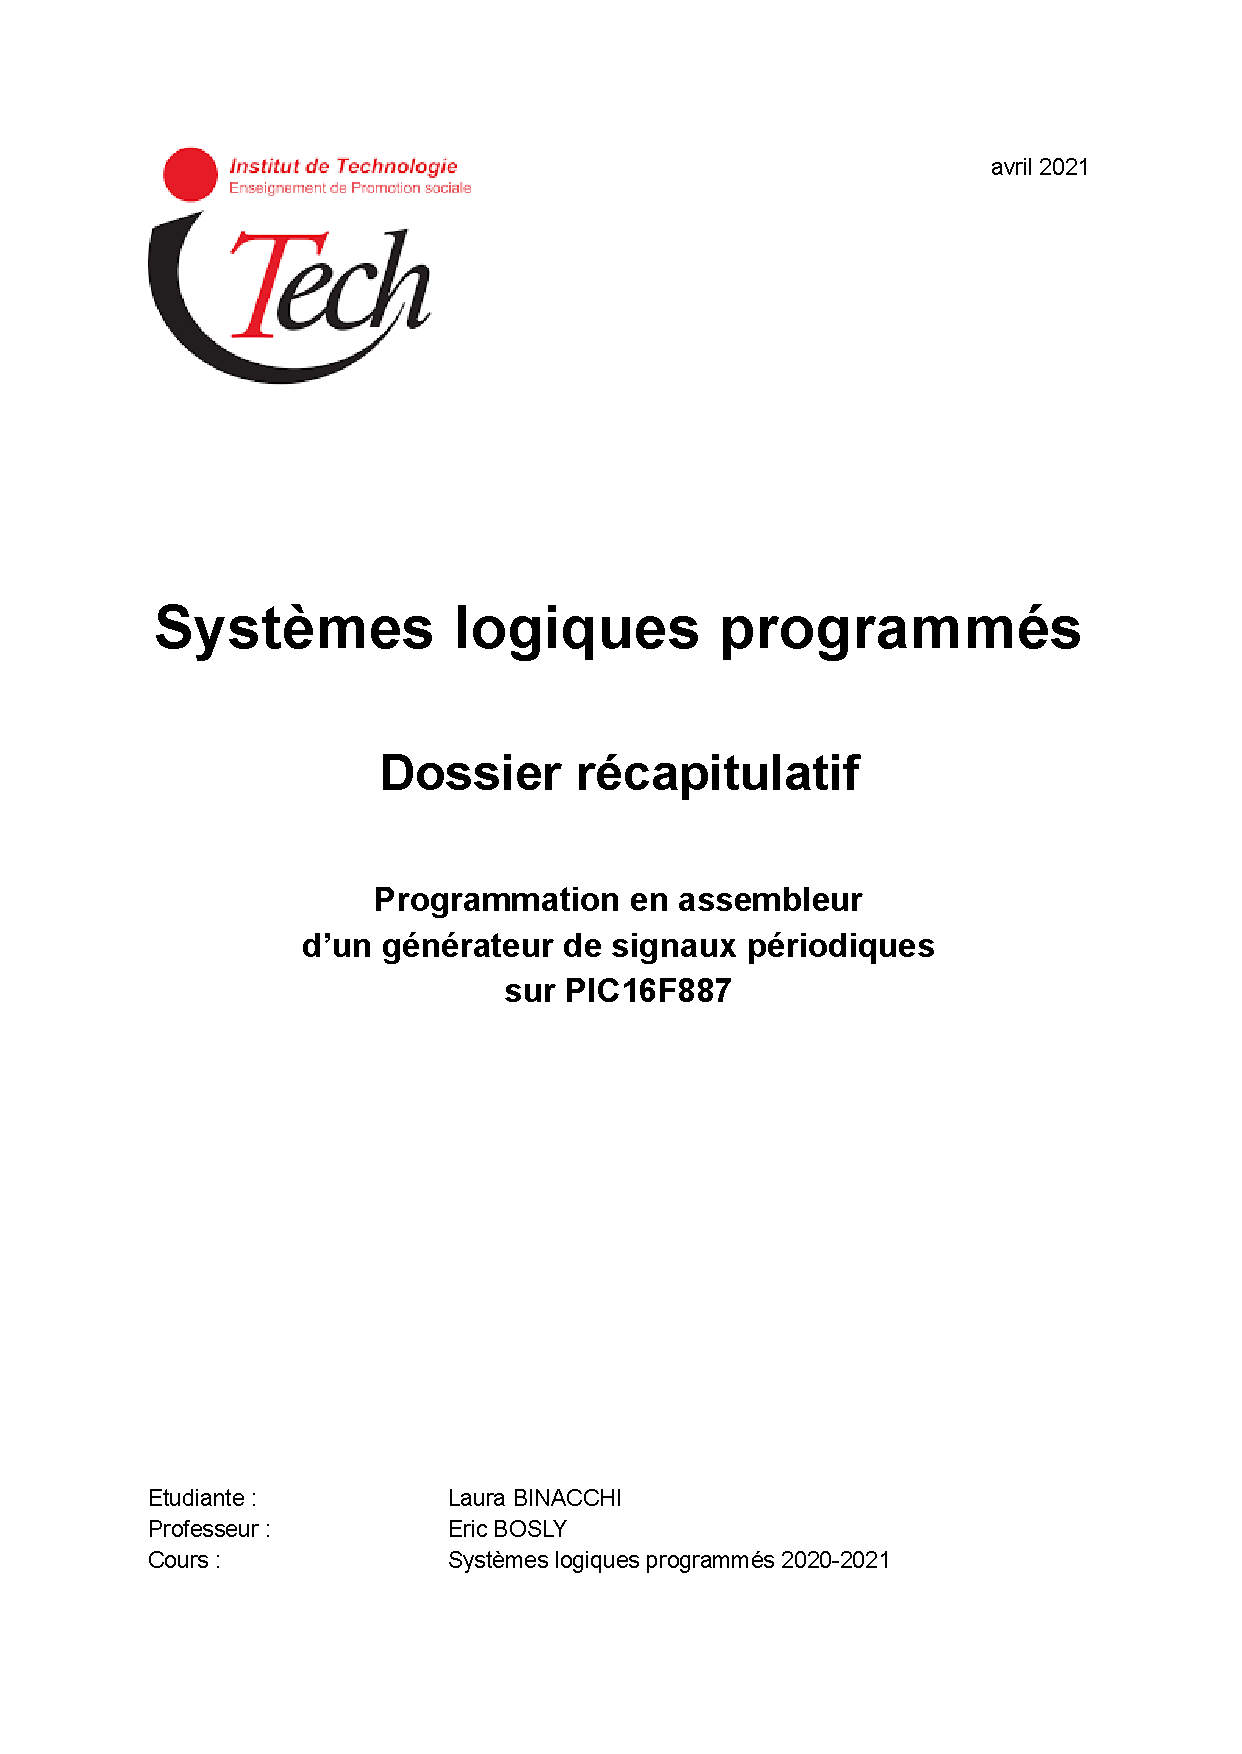
\includepdf[pages={1}]{pdg}
    \newpage
    \tableofcontents
    \newpage
    \pagenumbering{arabic}

    \section{Cahier des charges}
    \paragraph{}
    Sur base des modules élémentaires et exemples vus au cours (ports, interruptions, timers, CCP, SPI, I2C, ADC, LCD) développer sous MPLABX une application en langage d’assemblage sur PIC série 16F8xx ou 16F9xx ainsi que le modèle Proteus permettant de la simuler. L’application devra utiliser au moins une source d’interruptions, gérer un LCD et connecter au moins un circuit esclave en mode SPI ou I2C.

    \paragraph{}
    L’application permettra de générer un signal simple, carré ou triangulaire, de fréquence et rapport cyclique paramétrables. Le signal sera généré par l’intermédiaire d’un DAC 8 bits.

    \paragraph{}
    Les datasheets des PIC et des circuits nécessaires sont données, vous pouvez en choisir d’autres si vous le souhaitez et que cela se justifie. Vous ne devez évidemment pas utiliser tous les circuits, juste ceux nécessaires pour votre application. Une routine de conversion bianire / BCD est également donnée.

    \paragraph{}
    Les caractéristiques de l'applications sont données dans la liste ci-dessous. Vous avez le choix du dispositif de saisie (boutons, clavier, roue codeuse, dip switch, ...) et de la taille de l’écran, minimum 2x16 caractères. Vous pouvez faire plus que demandé, pas moins.
    \begin{itemize}[label=$\bullet$]
        \item Application : générateur de signaux
        \item PIC : 16F876A, 16F877A ou 16F887
        \item Bus : I2C
        \item Sortie signal : DAC 0808 connection directe au PIC
        \item Paramètres : fréquence, type et rapport cyclique du signal
        \item LCD : connection au bus I2C via IO expander 16 bits
    \end{itemize}

    \section{La description du projet et une brève analyse de celui-ci}
    \section{Une description du fonctionnement de votre programme}
    \section{Une justification des circuits et modules utilisés}
    \section{La configuration du microcontrôleur}
    \section{Les tests réalisés}
    \section{Les problèmes rencontrés}
    
\end{document}